% Taller 1 -- Perceptrón y Adaline. Compilar:
% tectonic -Z search-path=$HOME/repos/ud/maestria/mcic/.UniversidadDistrital-manual-marca/plantillas-latex informe_taller1.tex
% Las cifras salen de taller1_perceptron_adaline.ipynb ejecutado.
\documentclass[11pt,letterpaper]{article}
\usepackage{ud-informe}
\usepackage{amsmath}
\usepackage{qrcode}
\colorlet{udrojo}{udazul}
\definecolor{udrojoosc}{HTML}{0C6F96}

\renewcommand{\UDtitulo}{Perceptrón simple y Adaline}
\renewcommand{\UDsubtitulo}{Compuertas lógicas, Iris y autenticación de billetes}
\renewcommand{\UDtipo}{Taller 1 -- Informe}
\renewcommand{\UDasignatura}{Inteligencia Computacional Aplicada}
\renewcommand{\UDdocente}{Cesar Andrey Perdomo Charry}
\renewcommand{\UDestudiantes}{Juan Felipe Rodríguez Galindo -- 20261595004}
\renewcommand{\UDencabezado}{Taller 1 -- Perceptrón y Adaline}

\begin{document}
\UDportada

\section{Introducción}

En este taller implementé una neurona de una sola capa con dos modelos: el perceptrón simple, con las tres reglas de corrección de pesos del enunciado, y Adaline, con la regla delta. Los dos quedaron parametrizables (entradas, umbral, regla, $\alpha$, épocas) y se probaron en compuertas AND y OR de 2, 3 y 4 entradas y en dos conjuntos reales: Iris (Setosa contra el resto) y \textit{data\_banknote\_authentication}, con particiones 60-40, 70-30, 80-20 y 90-10. El enunciado pide scripts de MATLAB; los hice en Python (Jupyter), replicando la lógica de \textit{Dataset\_train\_test.mlx}.

Entregables: el cuaderno \texttt{taller1\_perceptron\_adaline.ipynb} ejecutado, \texttt{requirements.txt}, la carpeta \texttt{bibliografia/} con \textit{data\_banknote\_authentication.txt} (el cuaderno lee el archivo desde esa ruta) y este informe. Todo el desarrollo quedó grabado en video (sección~\ref{sec:ia}).

\section{Marco teórico}

\textbf{Perceptrón simple.} La entrada se aumenta con un 1 para que $w_0$ haga de sesgo: $X = [1, x_1, \dots, x_n]$. La neurona calcula $z = W \cdot X$ y responde $Y = 1$ si $z \ge \theta$, y $Y = 0$ en otro caso. Después de cada ejemplo los pesos se ajustan con $W^* = W + \Delta W$, usando una de tres reglas:
\begin{equation*}
\text{(1)}\ \Delta W = d\,X \qquad \text{(2)}\ \Delta W = (d - Y)\,X \qquad \text{(3)}\ \Delta W = \alpha\,(d - Y)\,X
\end{equation*}
El teorema de convergencia del perceptrón garantiza que las reglas 2 y 3 terminan en un número finito de pasos si las clases son linealmente separables. La regla 1 no usa el error: corrige igual cuando la respuesta es correcta.

\textbf{Adaline.} Usa la misma suma ponderada, pero el ajuste se hace con la salida \emph{lineal} $Y = W \cdot X$, sin escalón: $\Delta W = \alpha\,(d - Y)\,X$ (regla delta). Esto es descenso de gradiente sobre el error cuadrático, así que Adaline minimiza el MSE y no el número de errores. El escalón con umbral $\theta$ solo se usa para clasificar.

\section{Metodología}

\textbf{Entorno.} Python 3.12 con numpy, pandas y matplotlib; scikit-learn solo para cargar Iris. Todos los parámetros están en el diccionario \texttt{PARAMS} al inicio del cuaderno (tabla~\ref{tab:params}). Las clases \texttt{Perceptron} y \texttt{Adaline} reciben como argumentos el número de entradas, el umbral, la regla, $\alpha$, el máximo de épocas y, en Adaline, la tolerancia; los experimentos (compuertas, número de entradas, reglas, valores de $\alpha$, particiones y semilla) también se leen de \texttt{PARAMS}, así que cualquier corrida se cambia sin editar el código.

\begin{table}[H]
\centering
\caption{Parámetros de los experimentos (\texttt{PARAMS}).}\label{tab:params}
\begin{tabular}{lll}
\toprule
Parámetro & Perceptrón & Adaline \\
\midrule
Pesos iniciales & ceros & ceros \\
Umbral $\theta$ & 0 y 0,5 (compuertas); 0 (datasets) & 0,5 \\
Regla & 1, 2 y 3 & delta \\
$\alpha$ & 0,01; 0,1; 0,5; 1 & 0,001; 0,01; 0,05; 0,1 \\
Máximo de épocas & 100 & 200 \\
Criterio de parada & una época sin errores & cambio del MSE $< 10^{-6}$ o divergencia \\
Semilla de partición & 2021 & 2021 \\
Compuertas & AND, OR de 2, 3 y 4 entradas & AND, OR de 2, 3 y 4 entradas \\
Particiones & 60-40, 70-30, 80-20, 90-10 & 60-40, 70-30, 80-20, 90-10 \\
\bottomrule
\end{tabular}
\end{table}

\textbf{Compuertas.} Se generan todas las combinaciones de entradas binarias ($2^n$ filas) con \texttt{itertools.product}; la salida deseada es AND u OR de la fila.

\textbf{Particiones (puntos 4, 5, 10 y 11).} La función \texttt{particionar} hace lo mismo que \textit{Dataset\_train\_test.mlx}: fija la semilla, permuta los índices y corta según la proporción. El generador de numpy no produce la misma permutación que \texttt{randperm} de MATLAB, así que las particiones son equivalentes pero no idénticas. Iris tiene 150 muestras (50 Setosa = 1, 100 resto = 0). Banknote tiene 1372 muestras con 4 atributos (762 de clase 0 y 610 de clase 1); como sus escalas son distintas, se normaliza con la media y la desviación del entrenamiento y esas mismas estadísticas se aplican a la prueba. En Adaline también se normaliza Iris.

\section{Resultados}

\subsection{Perceptrón en compuertas (punto 3)}

La tabla~\ref{tab:epocas} resume las épocas hasta converger. Las reglas 2 y 3 convergen en todos los casos con 100\,\% de exactitud; la regla 1 llega siempre al máximo de 100 épocas.

\begin{table}[H]
\centering
\caption{Épocas hasta converger del perceptrón (100 = no convergió). Regla 3 con $\alpha = 0{,}1$.}\label{tab:epocas}
\begin{tabular}{llcccccc}
\toprule
& & \multicolumn{2}{c}{Regla 1} & \multicolumn{2}{c}{Regla 2} & \multicolumn{2}{c}{Regla 3} \\
\cmidrule(lr){3-4}\cmidrule(lr){5-6}\cmidrule(lr){7-8}
Compuerta & Entradas & $\theta=0$ & $\theta=0{,}5$ & $\theta=0$ & $\theta=0{,}5$ & $\theta=0$ & $\theta=0{,}5$ \\
\midrule
AND & 2 & 100 & 100 & 6 & 6 & 4 & 3 \\
AND & 3 & 100 & 100 & 7 & 7 & 3 & 4 \\
AND & 4 & 100 & 100 & 16 & 16 & 17 & 2 \\
OR & 2 & 100 & 100 & 4 & 4 & 4 & 2 \\
OR & 3 & 100 & 100 & 5 & 5 & 5 & 2 \\
OR & 4 & 100 & 100 & 6 & 6 & 6 & 3 \\
\bottomrule
\end{tabular}
\end{table}

Con la regla 1 los pesos solo crecen: en AND de 2 entradas terminan en $[100, 100, 100]$ y la exactitud queda en 25\,\% (AND-3: 12,5\,\%; AND-4: 6,25\,\%; OR-2: 75\,\%; OR-4: 93,75\,\%). La figura~\ref{fig:curvas} muestra los errores por época de las tres reglas en AND y OR de 2 entradas.

\begin{figure}[H]
\centering
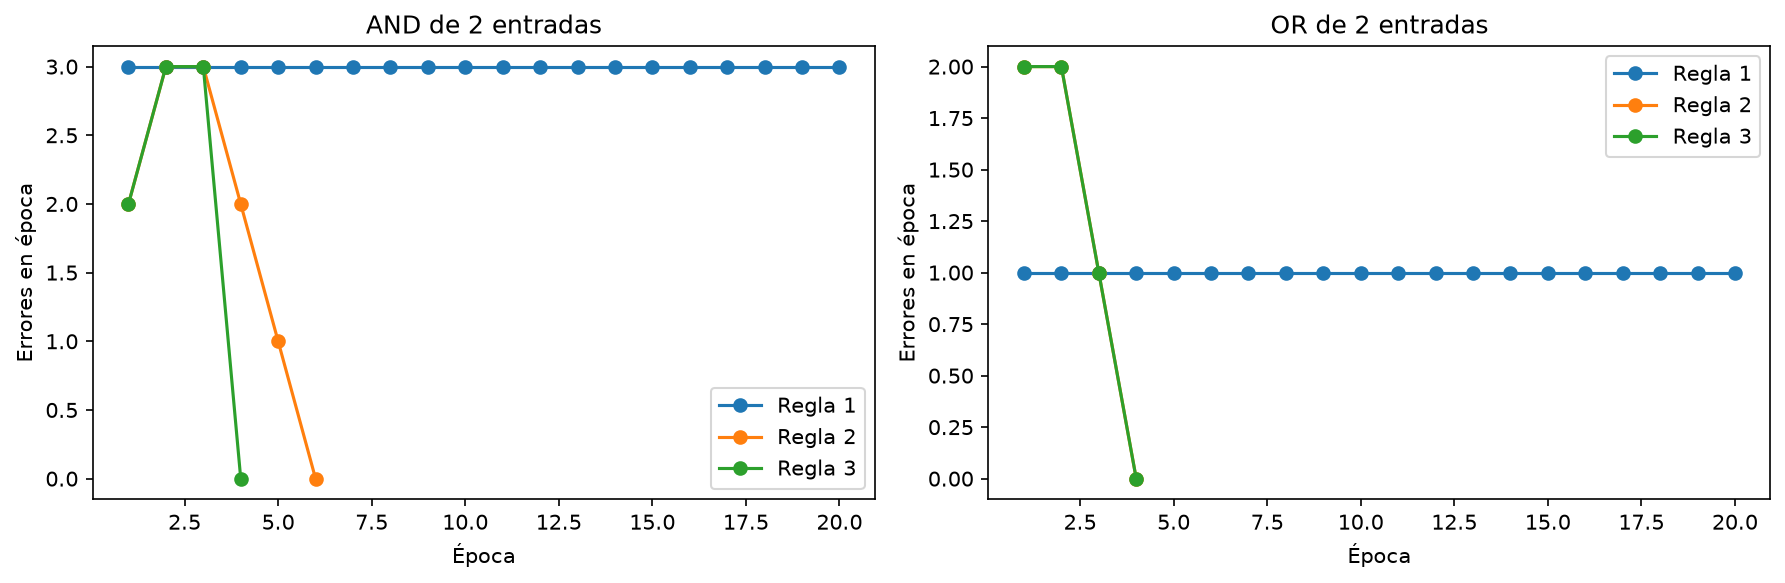
\includegraphics[width=\linewidth]{../figuras/perceptron_curvas_error.png}
\caption{Errores por época del perceptrón en AND y OR de 2 entradas ($\theta = 0$, $\alpha = 0{,}1$).}\label{fig:curvas}
\end{figure}

La tabla~\ref{tab:alfa} cruza $\alpha$ y $\theta$ en la regla 3.

\begin{table}[H]
\centering
\caption{Épocas de la regla 3 según $\alpha$ y el umbral $\theta$.}\label{tab:alfa}
\begin{tabular}{llcccccccc}
\toprule
& & \multicolumn{4}{c}{$\theta = 0$} & \multicolumn{4}{c}{$\theta = 0{,}5$} \\
\cmidrule(lr){3-6}\cmidrule(lr){7-10}
Compuerta & Entradas & 0,01 & 0,1 & 0,5 & 1 & 0,01 & 0,1 & 0,5 & 1 \\
\midrule
AND & 2 & 6 & 4 & 6 & 6 & 18 & 3 & 6 & 6 \\
AND & 3 & 7 & 3 & 7 & 7 & 14 & 4 & 7 & 7 \\
AND & 4 & 16 & 17 & 16 & 16 & 11 & 2 & 16 & 16 \\
OR & 2 & 4 & 4 & 4 & 4 & 13 & 2 & 4 & 4 \\
OR & 3 & 5 & 5 & 5 & 5 & 8 & 2 & 5 & 5 \\
OR & 4 & 6 & 6 & 6 & 6 & 6 & 3 & 6 & 6 \\
\bottomrule
\end{tabular}
\end{table}

\subsection{Perceptrón en datos reales (puntos 4 a 6)}

La tabla~\ref{tab:perc_datos} muestra el perceptrón en las cuatro particiones de cada conjunto. En Iris converge siempre; en banknote llega al máximo de épocas en todas las particiones, pero con exactitud de prueba alta.

\begin{table}[H]
\centering
\caption{Perceptrón (regla 3, $\theta = 0$) en Iris y banknote. El resultado es el mismo para los cuatro valores de $\alpha$.}\label{tab:perc_datos}
\begin{tabular}{lccccccc}
\toprule
& \multicolumn{3}{c}{Iris (Setosa / resto)} & \multicolumn{4}{c}{Banknote} \\
\cmidrule(lr){2-4}\cmidrule(lr){5-8}
Partición & Train / test & Épocas & Test & Train / test & Épocas & Train & Test \\
\midrule
60-40 & 90 / 60 & 2 & 100\,\% & 823 / 549 & 100 & 98,30\,\% & 97,27\,\% \\
70-30 & 105 / 45 & 2 & 100\,\% & 960 / 412 & 100 & 99,27\,\% & 99,03\,\% \\
80-20 & 120 / 30 & 2 & 100\,\% & 1097 / 275 & 100 & 98,91\,\% & 98,91\,\% \\
90-10 & 135 / 15 & 2 & 100\,\% & 1234 / 138 & 100 & 99,19\,\% & 98,55\,\% \\
\bottomrule
\end{tabular}
\end{table}

\subsection{Adaline (puntos 7 a 12)}

La tabla~\ref{tab:ada_comp} muestra la exactitud de Adaline en las compuertas y la figura~\ref{fig:mse} el MSE por época en OR de 2 entradas para distintos $\alpha$, incluidos 0,5 y 1 para ver el límite de estabilidad.

\begin{table}[H]
\centering
\caption{Exactitud de Adaline ($\theta = 0{,}5$) en compuertas según $\alpha$.}\label{tab:ada_comp}
\begin{tabular}{llcccc}
\toprule
Compuerta & Entradas & 0,001 & 0,01 & 0,05 & 0,1 \\
\midrule
AND & 2 & 75\,\% & 100\,\% & 100\,\% & 100\,\% \\
AND & 3 & 87,5\,\% & 87,5\,\% & 100\,\% & 100\,\% \\
AND & 4 & 93,75\,\% & 93,75\,\% & 93,75\,\% & 100\,\% \\
OR & 2 & 100\,\% & 100\,\% & 100\,\% & 100\,\% \\
OR & 3 & 100\,\% & 100\,\% & 87,5\,\% & 87,5\,\% \\
OR & 4 & 93,75\,\% & 93,75\,\% & 93,75\,\% & 93,75\,\% \\
\bottomrule
\end{tabular}
\end{table}

\begin{figure}[H]
\centering
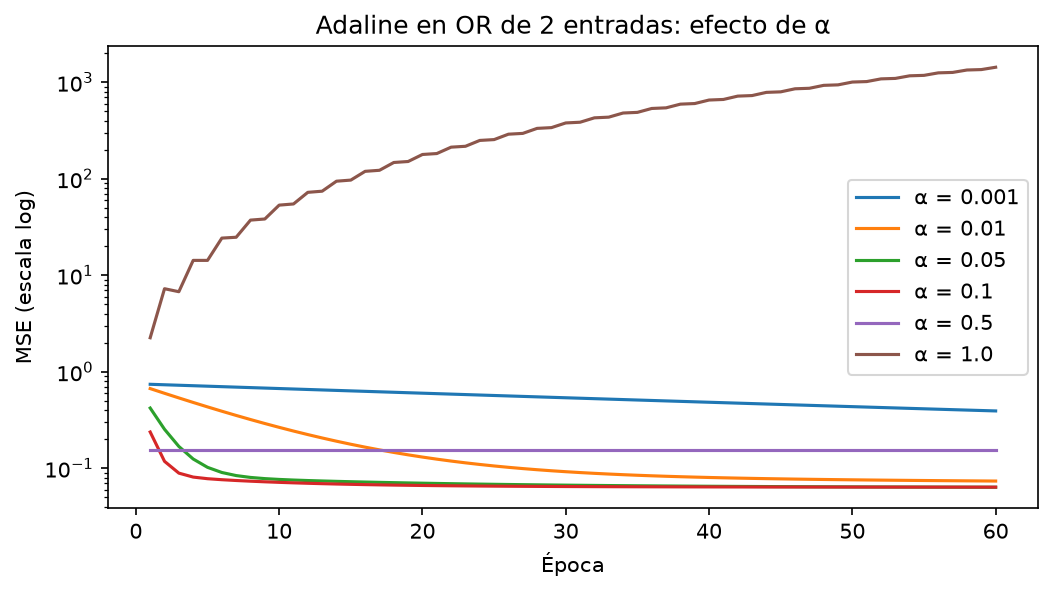
\includegraphics[width=0.8\linewidth]{../figuras/adaline_mse_alfa.png}
\caption{MSE por época de Adaline en OR de 2 entradas (60 épocas, escala logarítmica).}\label{fig:mse}
\end{figure}

La tabla~\ref{tab:ada_bn} muestra Adaline en las particiones de banknote: la exactitud de prueba varía entre 96,1\,\% y 97,5\,\% y ningún $\alpha$ es mejor en todas. Después de 60 épocas, el MSE en OR-2 es 0,393 con $\alpha = 0{,}001$, 0,074 con 0,01 y 0,064 con 0,05 y 0,1. Con $\alpha = 0{,}5$ se queda fijo en 0,156 desde la primera época y con $\alpha = 1$ crece hasta 1428.

\begin{table}[H]
\centering
\caption{Exactitud de prueba de Adaline en banknote según $\alpha$ (en Iris es 100\,\% en todos los casos salvo 98,3\,\% con $\alpha=0{,}1$ en 60-40).}\label{tab:ada_bn}
\begin{tabular}{lcccc}
\toprule
Partición & 0,001 & 0,01 & 0,05 & 0,1 \\
\midrule
60-40 & 96,54\,\% & 96,36\,\% & 96,54\,\% & 97,09\,\% \\
70-30 & 96,36\,\% & 96,12\,\% & 97,09\,\% & 97,33\,\% \\
80-20 & 96,73\,\% & 97,45\,\% & 97,09\,\% & 97,09\,\% \\
90-10 & 96,38\,\% & 96,38\,\% & 97,10\,\% & 96,38\,\% \\
\bottomrule
\end{tabular}
\end{table}

\subsection{Comparación}

La tabla~\ref{tab:comp} reúne la mejor exactitud de prueba de cada modelo por partición.

\begin{table}[H]
\centering
\caption{Mejor exactitud de prueba por partición (máximo sobre $\alpha$).}\label{tab:comp}
\begin{tabular}{lcccc}
\toprule
Partición & Perceptrón Iris & Adaline Iris & Perceptrón banknote & Adaline banknote \\
\midrule
60-40 & 100\,\% & 100\,\% & 97,27\,\% & 97,09\,\% \\
70-30 & 100\,\% & 100\,\% & 99,03\,\% & 97,33\,\% \\
80-20 & 100\,\% & 100\,\% & 98,91\,\% & 97,45\,\% \\
90-10 & 100\,\% & 100\,\% & 98,55\,\% & 97,10\,\% \\
\bottomrule
\end{tabular}
\end{table}

\section{Análisis}

\textbf{La regla 1 no aprende.} $\Delta W = d\,X$ no depende de la respuesta $Y$: cada ejemplo con $d = 1$ suma su entrada a los pesos y los ejemplos con $d = 0$ no restan nada. Los pesos solo crecen y la neurona termina respondiendo 1 para todas las entradas; por eso su exactitud es exactamente la proporción de unos de la compuerta (25\,\% en AND-2, 75\,\% en OR-2). Con $\theta = 0{,}5$ pasa lo mismo.

\textbf{El efecto de $\alpha$ depende del umbral.} Con $\theta = 0$ y pesos iniciales en cero, todos los pesos son múltiplos de $\alpha$, así que el signo de $z$ no cambia al escalar y la frontera es la misma: casi todas las columnas de $\theta = 0$ en la tabla~\ref{tab:alfa} coinciden con la regla 2. Las diferencias en $\alpha = 0{,}1$ (4 épocas en AND-2, 17 en AND-4) vienen del redondeo de punto flotante en los empates $z = 0$: $0{,}1 + 0{,}2 - 0{,}3$ no da exactamente cero. Con $\theta = 0{,}5$ el umbral fija una escala y $\alpha$ sí importa: con 0,01 los pasos son pequeños frente al umbral y AND-2 tarda 18 épocas; con 0,1 tarda 3; con 0,5 y 1 los pasos son tan grandes que el umbral deja de pesar y se repiten las épocas de $\theta = 0$.

\textbf{Iris y banknote.} Setosa es linealmente separable del resto, y el perceptrón converge en 2 épocas con 100\,\% en prueba en todas las particiones. Banknote no es perfectamente separable: el perceptrón nunca termina una época sin errores y siempre llega a 100 épocas, pero la frontera que encuentra clasifica entre 97,3\,\% y 99,0\,\% en prueba. Como los pesos parten de cero y $\theta = 0$, $\alpha$ tampoco cambia el resultado aquí. La partición 60-40 es la más baja porque tiene menos datos para entrenar.

\textbf{Adaline.} Al minimizar el MSE, Adaline busca la recta de mínimos cuadrados y no la que separa sin errores, así que no siempre clasifica bien todas las filas aunque la compuerta sea separable (OR-4 se queda en 93,75\,\% con todos los $\alpha$). Un $\alpha$ muy pequeño no alcanza a bajar el error en 200 épocas (AND-2 con 0,001: 75\,\%). La figura~\ref{fig:mse} muestra el límite de estabilidad: hasta 0,1 el MSE baja al mínimo de 0,064; con 0,5 la actualización oscila entre dos valores y el MSE no se mueve; con 1 los pesos se disparan y el error diverge.

\textbf{Perceptrón contra Adaline.} En Iris los dos llegan a 100\,\%. En banknote el perceptrón queda por encima en las cuatro particiones (tabla~\ref{tab:comp}): Adaline converge en pocas épocas al mínimo del MSE, pero ese mínimo no es la frontera con menos errores de clasificación.

\section{Conclusiones}

\begin{enumerate}
\item Las reglas 2 y 3 del perceptrón resolvieron todas las compuertas AND y OR de 2, 3 y 4 entradas (regla 2: AND en 6, 7 y 16 épocas; OR en 4, 5 y 6). La regla 1 no convergió en ninguna, porque sin el término de error los pesos solo crecen y la neurona responde 1 para todo.
\item Con $\theta = 0$ y pesos en cero, $\alpha$ solo escala los pesos y no cambia la frontera. Con $\theta = 0{,}5$ sí importa: en AND-2, $\alpha = 0{,}01$ necesitó 18 épocas y $\alpha = 0{,}1$, 3.
\item En Iris (Setosa contra el resto) el perceptrón convergió en 2 épocas con 100\,\% en prueba. En banknote no convergió en 100 épocas, pero alcanzó entre 97,3\,\% y 99,0\,\% en prueba.
\item Adaline necesita un $\alpha$ pequeño: en OR-2, con 0,05 y 0,1 llega al MSE mínimo (0,064), con 0,5 se estanca y con 1 diverge. Como minimiza el MSE y no los errores, no clasifica perfecto todas las compuertas (OR-4: 93,75\,\%).
\item En banknote el perceptrón superó a Adaline en las cuatro particiones (mejor caso 99,0\,\% contra 97,5\,\%); en Iris los dos llegaron a 100\,\%.
\end{enumerate}

\section{Declaración de uso de IA}\label{sec:ia}

Usé Claude (Anthropic) para revisar y corregir errores y para redactar este informe a partir de los resultados del cuaderno. Todo el desarrollo quedó grabado (cerca de 2 horas y 40 minutos):

\begin{center}
\qrcode[height=3.2cm,nolink]{https://youtu.be/TNVHhuWUC0g}\\[0.6em]
\url{https://youtu.be/TNVHhuWUC0g}
\end{center}

\end{document}
